% !TEX root = ../Tesis_NataliaOpazo.tex

El \'area de estudio comprende la totalidad del globo (figura \ref{fig:Grilla4}). Se ver\'a con especial atenci\'on zonas regionales del oc\'eano (HNLC) que se encuentran definidas en la tabla \ref{tabla:Area1} y que gr\'aficamente podemos apreciar en la imagen
\ref{fig:Grilla4}. 

\begin{figure}[H]
\centering
  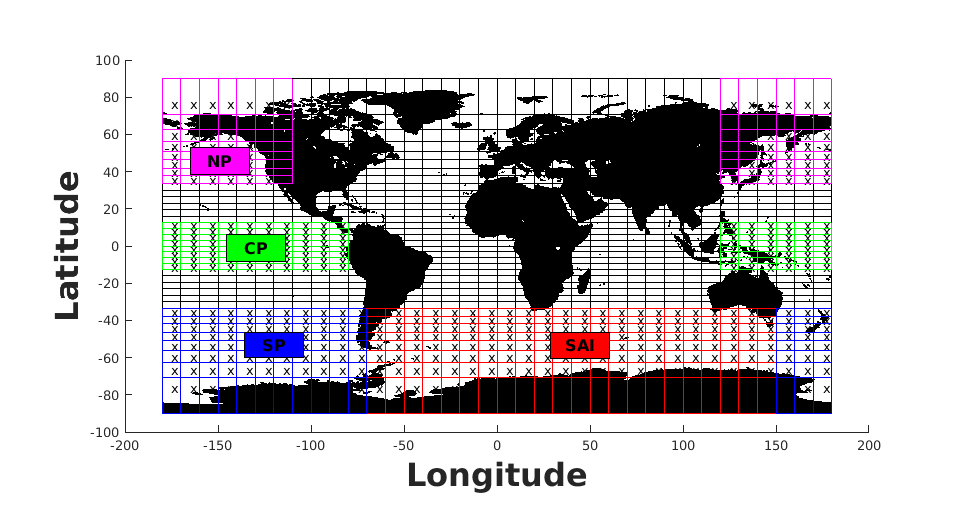
\includegraphics[width=0.9\textwidth]{mapa.png}
  \caption[Grilla global y regional de campos de flujo de polvo]{Grilla cGenie con la especificaci\'on de las zonas HNLC a simular: Pac\'ifico norte (NP), Pac\'ifico Sur (SP), P\'acifico Central (CP) y Atl\'antico/Índico Sur (SAI).}
  \label{fig:Grilla4}
\end{figure} 

El detalle de las distintas regiones oce\'anicas se presentan en la tabla a continuaci\'on. \newpage

\begin{table}[H]
\begin{center}
\begin{tabular}{l|l|l|l|l}
\hline
\multirow{2}{1cm}{ Zona}& Latitud & Longitud &Puntos & \'Area \\
 & cuadrante & cuadrante & de grilla & total  ($km^{2}$)\\
\hline \hline
Atlántico/Índico del Sur (SAI)& -90 a -33.7490 & -70 a 150 & 176&  6.9268e+07 \\ \hline
Pac\'ifico Sur (SP) & -90 a -33.7490 & -180 a -70 y 150 a 180& 112 & 4.4080e+07  \\ \hline
Pac\'ifico Norte (NP) & 33.7490 a 90 &  -180 a -110 y 120 a 180 & 104 & 4.0931e+07\\ \hline
Pac\'ifico Central (CP) & -12.8396 a 12.8396 & -180 a -80 y 120 a 180 & 128 & 5.0377e+07 \\ \hline
\end{tabular}
\caption{Caracter\'isticas de las regiones oce\'anicas simuladas en cGENIE.}
\label{tabla:Area1}
\end{center}
\end{table}
